\documentclass{article}
\usepackage{graphicx} % Required for inserting images
\usepackage{fancyvrb}
\usepackage{listings}
\usepackage{color}

\definecolor{dkgreen}{rgb}{0,0.6,0}
\definecolor{gray}{rgb}{0.5,0.5,0.5}
\definecolor{mauve}{rgb}{0.58,0,0.82}

\lstset{frame=tb,
  language=Java,
  aboveskip=3mm,
  belowskip=3mm,
  showstringspaces=false,
  columns=flexible,
  basicstyle={\small\ttfamily},
  numbers=none,
  numberstyle=\tiny\color{gray},
  keywordstyle=\color{blue},
  commentstyle=\color{dkgreen},
  stringstyle=\color{mauve},
  breaklines=true,
  breakatwhitespace=true,
  tabsize=3
}

\lstdefinestyle{outputStyle}{
  frame=tb,                   % Cornice sopra e sotto
  language=Python,            % Lingua, nel caso ci siano parole chiave
  aboveskip=3mm,
  belowskip=3mm,
  showstringspaces=false,
  columns=flexible,
  basicstyle={\footnotesize\ttfamily}, % Ridotto a \footnotesize
  numbers=none,               % Nessun numero di riga
  keywordstyle=\color{blue},  % Colore delle parole chiave
  commentstyle=\color{dkgreen}, % Colore dei commenti
  stringstyle=\color{mauve},  % Colore delle stringhe
  breaklines=true,            % Spezza automaticamente le righe lunghe
  breakatwhitespace=true,     % Spezza sugli spazi
  tabsize=3                   % Dimensione del tab
}


\title{Relazione progetto di Reti di Telecomunicazione}

\author{Matte Bagnolini : 0001071301}
\date{Dicembre 2024}

\begin{document}

\maketitle

\newpage

\tableofcontents

\newpage

\section{Introduzione}

Per questo progetto ho deciso di affrontare la traccia 2, cioè l'implementazione in Python di un protocollo di routing semplice. Ho scelto di implementare il Link-State routing protocol, che ha lo scopo di permettere ad ogni router di costruire una mappa di connettività del network di cui fa parte. \\
Ho deciso di implementare questo protocollo poichè riesce a superare alcuni problemi (come Count to Infinity e Bouncing effect) di Distance Vector Routing, che è l'altro principale protocollo di routing.

\newpage

\section{Requisiti}
Di seguito vengono specificati i requisiti per utilizzare l'applicativo:
\begin{itemize}
    \item Interprete per Python 3.*
    \item Modulo \texttt{networkX} per la gestione dei grafi di rete.
\end{itemize}
Le dipendenze sono comununque specificate nel file \texttt{requirements.txt}, da cui è possibile installare i moduli sopra citati.

\newpage

\section{Funzionamento del sistema}
Il sistema complessivo è suddiviso in 3 classi principali: \texttt{Node}, \texttt{Router} e \texttt{Network}. \\
La classe \texttt{Network} ha il compito di creare connessioni tra i router e gestire il corretto funzionamento del protocollo Link-State Routing, permettendo ai router di scambiarsi i Link State Packet e di calcolare i percorsi minimi e le tabelle di routing.\\

\subsection{Classe \texttt{Node}}
La classe \texttt{Node} rappresenta un generico nodo nella rete. Ognuno di questi nodi mantiene in memoria un grafo che ne rappresenta le proprie connessioni con altri nodi della network.\\
Su oggetti di questa classe è possibile chiamare il metodo \texttt{add\_edge(node\_id, distance)}, che permette di creare un arco tra due nodi.\\
Questa classe è stata creata per essere ereditata dalla classe \texttt{Router}, rendendo il codice più modulare.

\subsection{Classe \texttt{Router}}
Questa classe, che eredita dalla classe \texttt{Node}, rappresenta un router all'interno della rete. Ogni router mantiene in memoria, oltre al grafo delle proprie connessioni (ereditato da Node), il grafo completo della rete (che viene costruito progressivamente all'arrivo dei link state packet) e la routing table (anch'essa costruita una volta che il grafo di rete è completo).\\
Ogni router simula la ricezione (e l'invio) dei Link State Packet attraverso il metodo \texttt{receive\_link\_state\_packet(router)}. Questa funzione aggiorna il grafo di rete, aggiungendo le connessioni del router inviato come parametro. Di conseguenza, una volta ricevuti pacchetti da tutti gli altri router, il grafo di rete può ritenersi completo.\\
Quando il grafo è completo, può essere chiamato il metodo \texttt{calculate\_shortest\_path()}, che utilizza l'algoritmo di Dijkstra per calcolare il percorso minimo dal router sorgente ad ogni altro router della rete. Inoltre, viene anche compilata la routing table attraverso la tabella delle precedenze (calcolata sempre con Dijkstra).\\
Per visualizzare la tabella di routing si utilizza il metodo \texttt{print\_routing\_table()}.

\subsection{Classe \texttt{Network}}
Questa classe ha il compito di gestire i router della rete. Mantiene in memoria una lista dei router attivi, aggiunti tramite il metodo \texttt{add\_router(router)}.\\
Con il metodo \texttt{connect\_routers(router1, router2)}, permette ai due router di creare una connessione (cioè un arco tra i due nodi).\\
Questa classe gestisce anche la comunicazione tra router. Con il metodo \texttt{send\_link\_state\_packets()} permette ad ogni router di inviare il proprio grafo di connessioni agli altri, per creare il grafo di rete.\\
Una volta che il grafo di rete completo è disponibile in ogni router, può essere chiamato il metodo \texttt{calculate\_shortest\_paths()}, dove ogni router calcola il proprio percorso minimo e compila la propria tabella di routing.\\
Infine, per stampare tutte le tabelle di routing, può essere chiamato il metodo \texttt{print\_routing\_tables()}.

\newpage

\section{Guida Utente}
Nel file \texttt{main.py} è possibile definire una propria topologia di rete e simulare il Link-State Routing protocol.\\
\\
Si inizia creando un'istanza della classe network:

\begin{lstlisting}
    nw = Network()
\end{lstlisting}

Si definiscono poi i router che vogliamo includere nella rete:
\begin{lstlisting}
    rA = Router("A")
    rB = Router("B")
    rC = Router("C")
    rD = Router("D")
    rE = Router("E")
    rF = Router("F")
\end{lstlisting}

Aggiungiamo questi router alla rete:
\begin{lstlisting}
    nw.add_router(rA)
    nw.add_router(rB)
    nw.add_router(rC)
    nw.add_router(rD)
    nw.add_router(rE)
    nw.add_router(rF)
\end{lstlisting}

Connettiamo i router, specificando i pesi di ogni connessione:
\begin{lstlisting}
    nw.connect_routers(rA, rC, 5)
    nw.connect_routers(rA, rB, 2)
    nw.connect_routers(rA, rD, 1)
    nw.connect_routers(rB, rD, 2)
    nw.connect_routers(rB, rC, 3)
    nw.connect_routers(rC, rF, 5)
    nw.connect_routers(rC, rD, 3)
    nw.connect_routers(rC, rE, 1)
    nw.connect_routers(rD, rE, 1)
    nw.connect_routers(rE, rF, 2)
\end{lstlisting}
\newpage
A questo punto, il grafo di rete corrispondente è questo:
\begin{figure}[htp]
    \centering
    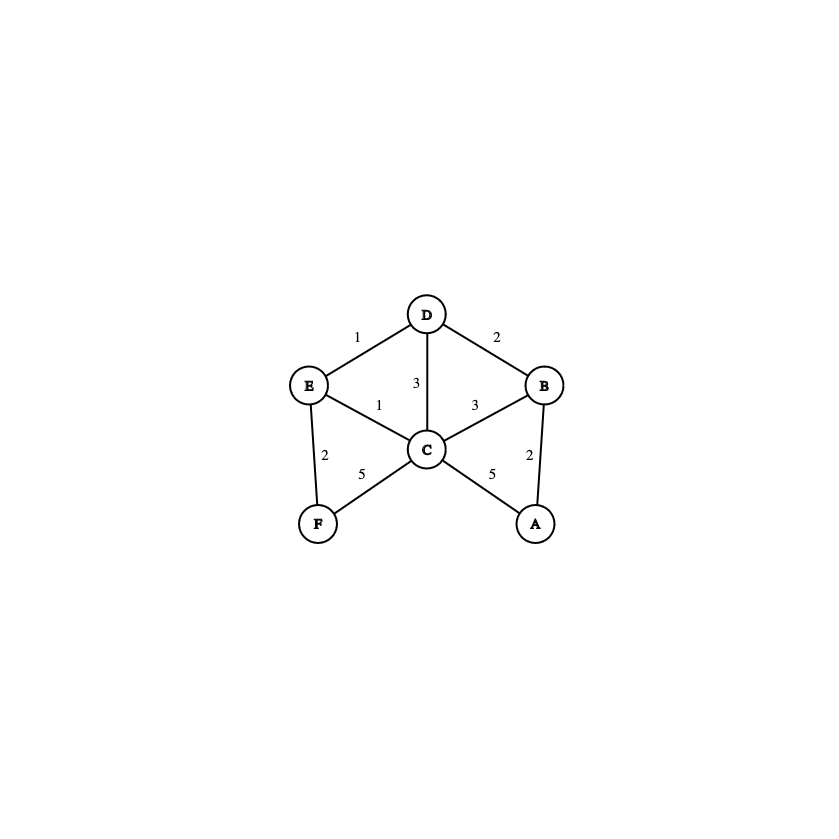
\includegraphics[width=10cm]{graph1.png}
    \caption{grafo di rete}
    \label{fig:grafo di rete}
\end{figure}

Simuliamo l'invio e la ricezione dei pacchetti link state:
\begin{lstlisting}
    nw.send_link_state_packets()
\end{lstlisting}

Dopo la chiamata a questo metodo, ogni router ha ottenuto il grafo di rete completo, quindi possiamo calcolare i percorsi minimi e le tabelle di routing:
\begin{lstlisting}
    nw.calculate_shortest_paths()
\end{lstlisting}

Ora le tabelle di routing sono compilate correttamente, quindi possiamo stamparle. Possiamo decidere se stampare la tabella di routing di uno specifico router
\begin{lstlisting}
    rA.print_routing_table()\end{lstlisting}
oppure stamparle tutte insieme:
\begin{lstlisting}
    nw.print_routing_tables()
\end{lstlisting}

\newpage
L'output generato è il seguente:
\begin{lstlisting}[style=OutputStyle]
    ----------------------------------------------
Routing table for router A:
Node A
         Cost: 0         Next hop: 
Node C
         Cost: 5         Next hop: C
Node B
         Cost: 2         Next hop: B
Node D
         Cost: 4         Next hop: B
Node F
         Cost: 7         Next hop: B
Node E
         Cost: 5         Next hop: B
----------------------------------------------
----------------------------------------------
Routing table for router B:
Node A
         Cost: 2         Next hop: A
Node B
         Cost: 0         Next hop: 
Node C
         Cost: 3         Next hop: C
Node D
         Cost: 2         Next hop: D
Node F
         Cost: 5         Next hop: D
Node E
         Cost: 3         Next hop: D
----------------------------------------------
----------------------------------------------
Routing table for router C:
Node A
         Cost: 5         Next hop: A
Node C
         Cost: 0         Next hop: 
Node B
         Cost: 3         Next hop: B
Node D
         Cost: 2         Next hop: E
Node F
         Cost: 3         Next hop: E
Node E
         Cost: 1         Next hop: E
----------------------------------------------
----------------------------------------------
Routing table for router D:
Node A
         Cost: 4         Next hop: B
Node D
         Cost: 0         Next hop: 
Node C
         Cost: 2         Next hop: E
Node B
         Cost: 2         Next hop: B
Node F
         Cost: 3         Next hop: E
Node E
         Cost: 1         Next hop: E
----------------------------------------------
----------------------------------------------
Routing table for router E:
Node A
         Cost: 5         Next hop: D
Node E
         Cost: 0         Next hop: 
Node C
         Cost: 1         Next hop: C
Node B
         Cost: 3         Next hop: D
Node D
         Cost: 1         Next hop: D
Node F
         Cost: 2         Next hop: F
----------------------------------------------
----------------------------------------------
Routing table for router F:
Node A
         Cost: 7         Next hop: E
Node F
         Cost: 0         Next hop: 
Node C
         Cost: 3         Next hop: E
Node B
         Cost: 5         Next hop: E
Node D
         Cost: 3         Next hop: E
Node E
         Cost: 2         Next hop: E
----------------------------------------------
\end{lstlisting}
\newpage

\section{Considerazioni}
È stato descritto la semplicità di creare una propria rete per simulare il protocollo Link-State Routing. Tuttavia questa simulazione non prevede l'effettivo invio di pacchetti Link State, ma semplicemente lo scambio di informazioni (i grafi di connessione) tra router gestito dalla classe \texttt{Network}. L'implementazione di un protocollo che preveda lo scambio di pacchetti sarebbe possibile ad esempio attraverso l'uso di socket per l'invio di messaggi con TCP o UDP.\\
Inoltre non esiste un vero e proprio pacchetto link state. Quello che viene scambiato è semplicemente un grafo che descrive le connessioni pesate di ogni router, senza altri controlli (ad esempio tramite il sequence number).\\
Sarebbe quindi interessante e opportuno modificare questa semplice implementazione per fare uso di socket e pacchetti veri e propri.
\end{document}
